\documentclass[a4j,11pt]{jsarticle}
\usepackage{semi}


\begin{document}
\begin{flushright} % 右揃え
2018 年 8 月3 日

阿部 希駿

 城 綾佳
\end{flushright}
\begin{center} % センタリングZ
\Large{夏合宿しおり}
\end{center}

\section{日程} % 第 1 章
\label{sec:start} % 第 1 章のラベル(後で参照する際に使います)
平成30年 9/3(月)\verb|~|9/5(水)     2泊3日

 
\section{集合} % 第 2 章
\label{sec:end} % 第 2 章のラベル
日程:9月3日(月)

時間:12:20

場所:東京駅B1「銀の鈴広場」

帰りは伊東駅で流れ解散にしようと思っています.

\begin{figure}[H]
\begin{center}
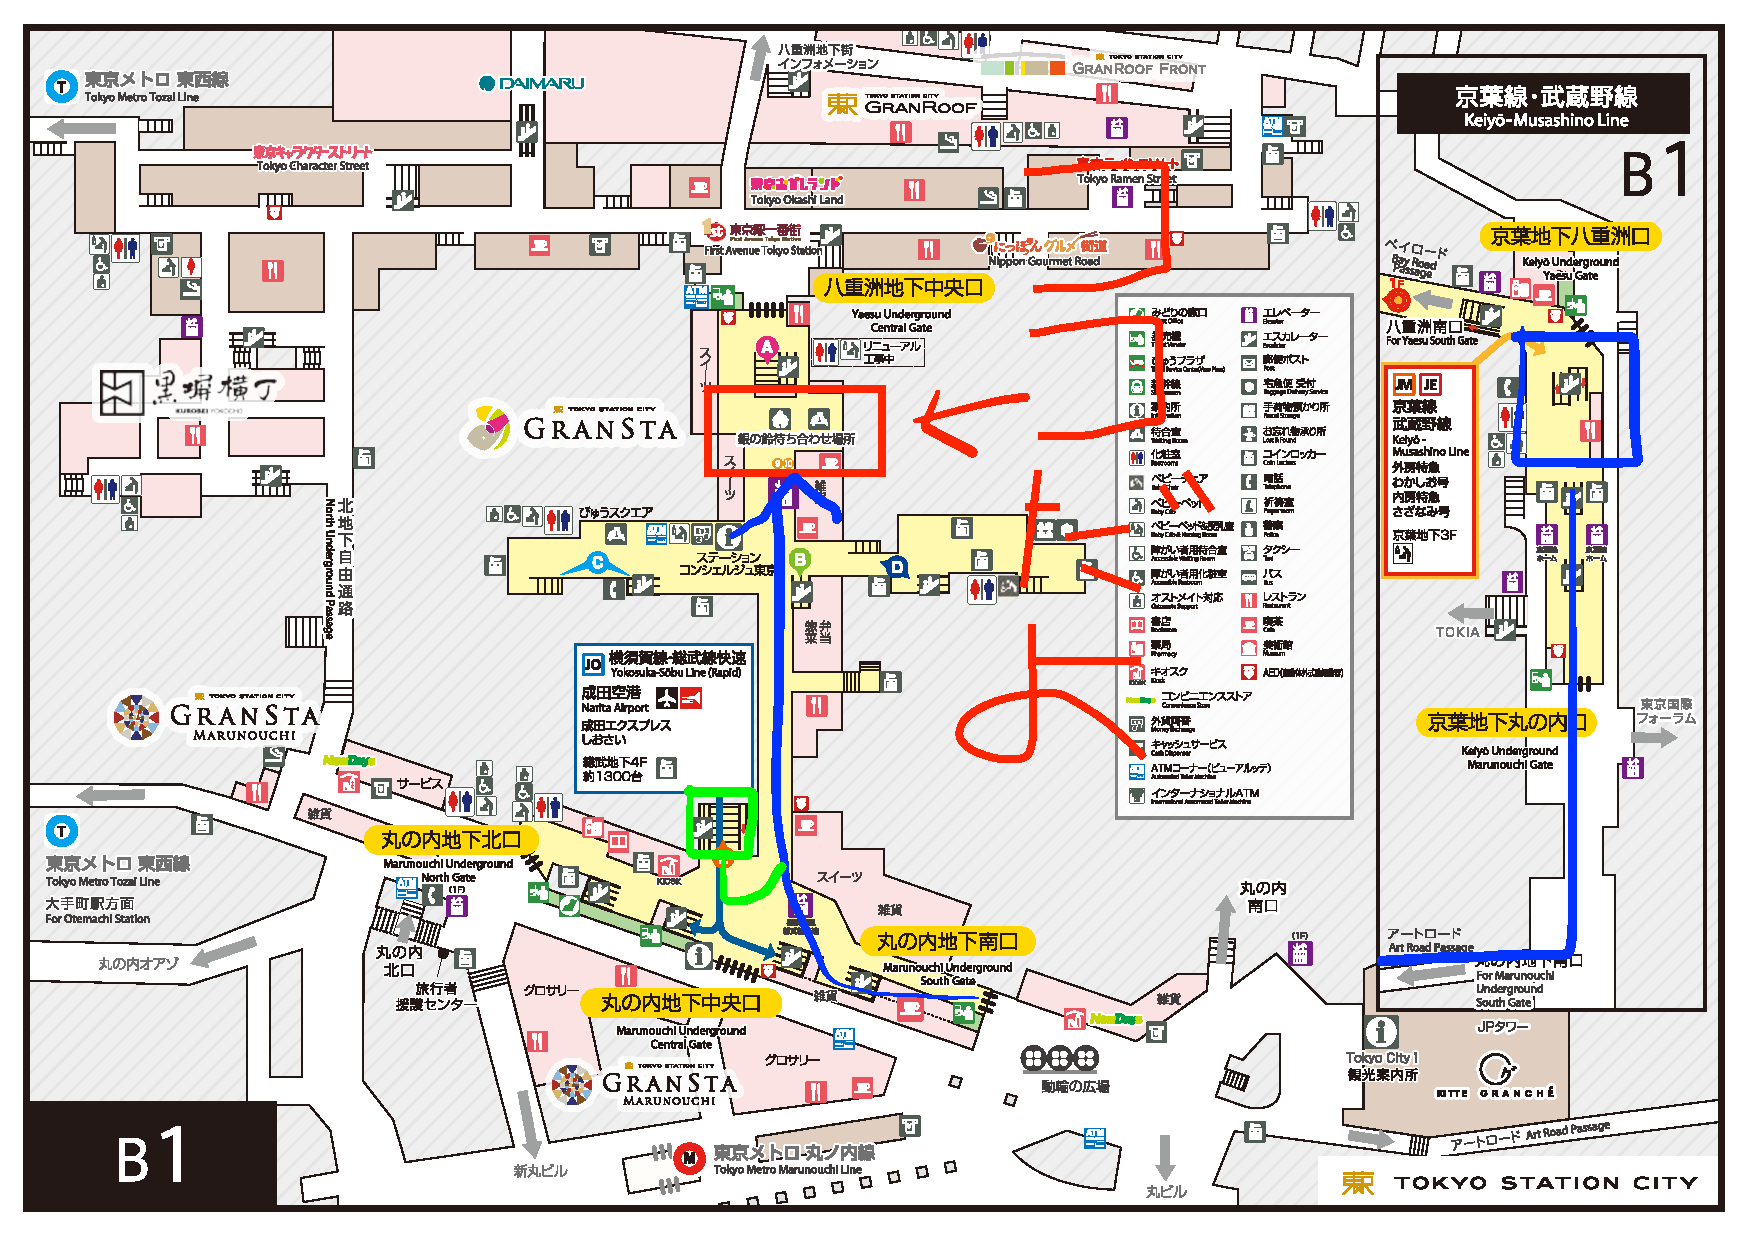
\includegraphics[width=85mm]{syuugo1.pdf}
\end{center}
\caption{集合場所}
\label{fig:2}
\end{figure}

\begin{figure}[H]
\begin{center}
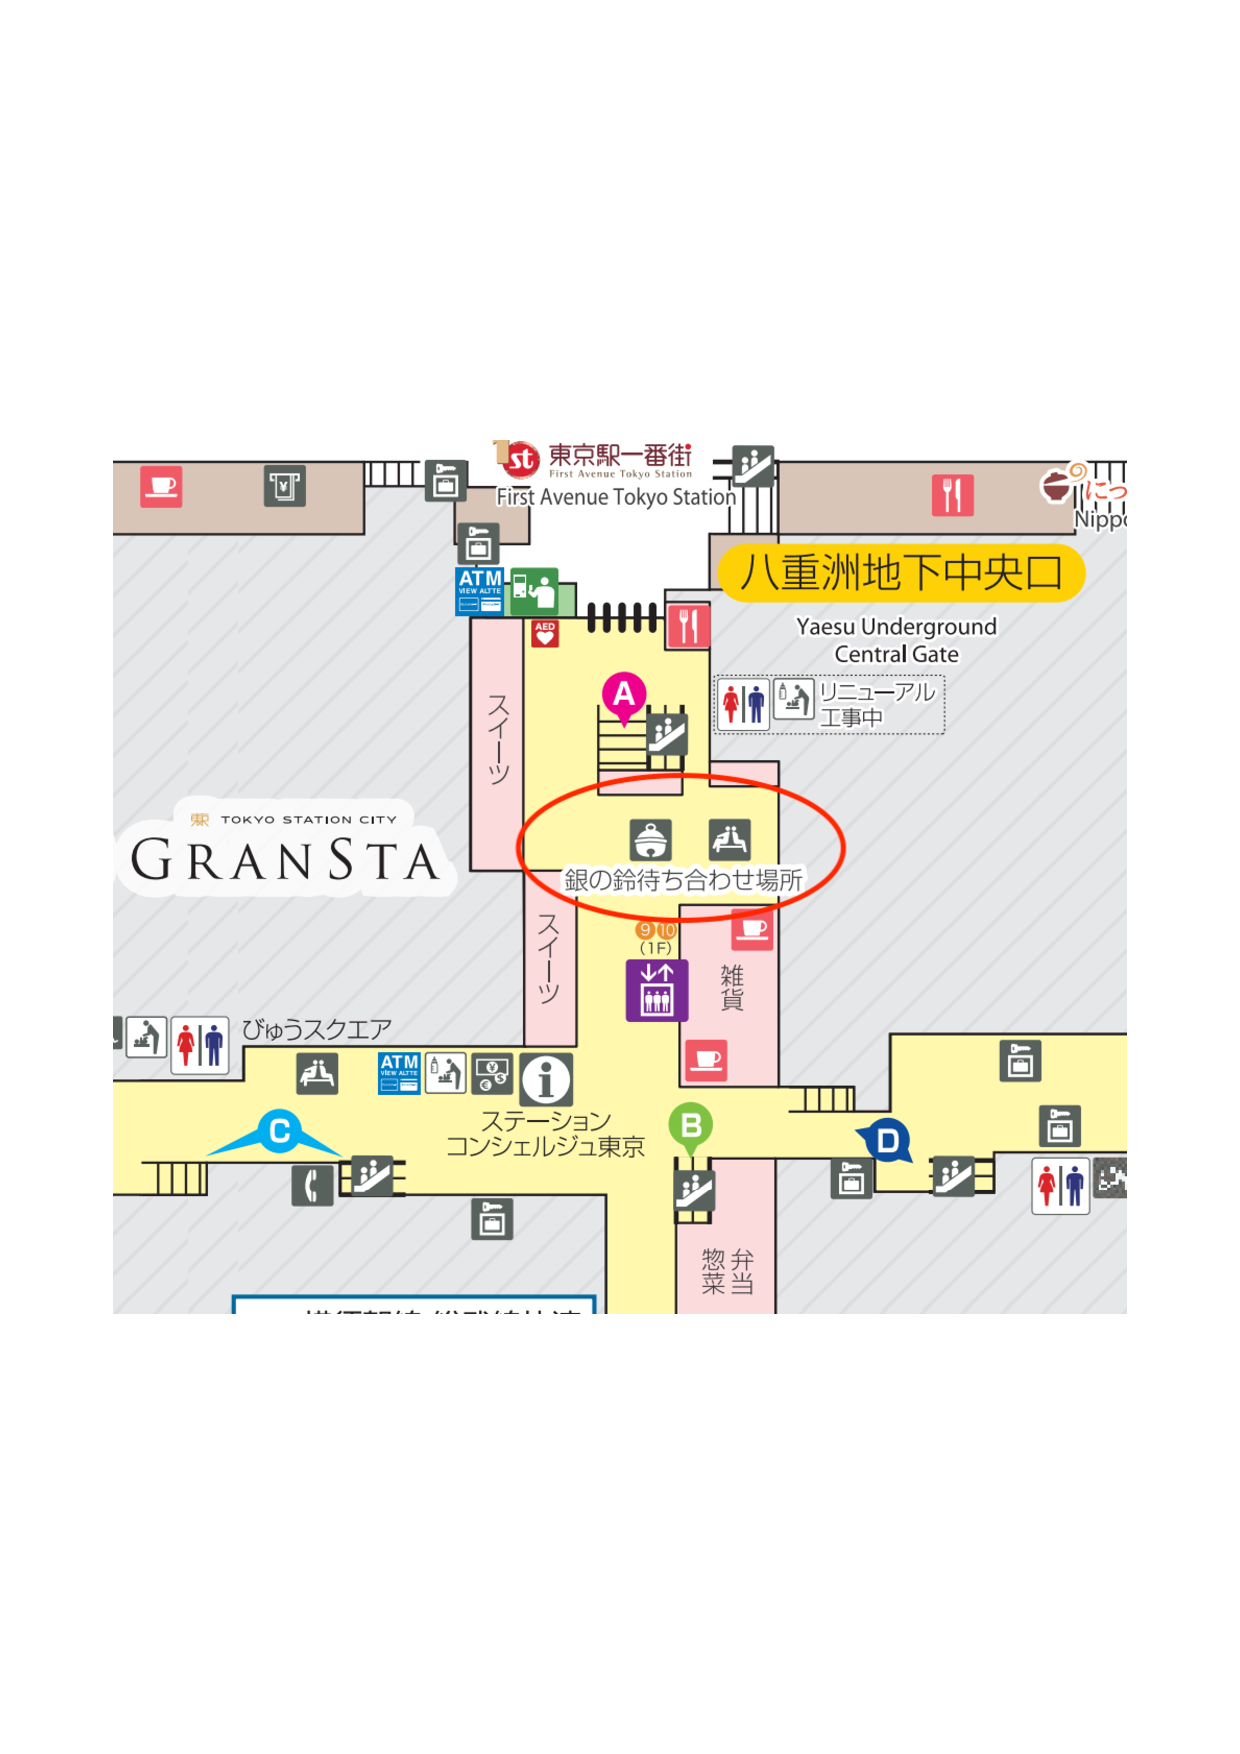
\includegraphics[mediaboxonly=/CropBox,width=85mm]{syuugoukakudai.pdf}
\end{center}
\caption{集合場所拡大図}
\label{fig:2}
\end{figure}

\section{予算} 
\label{sec:end} 
宿泊代 15,000円(事前に徴収)

昼食代

交通費

東京-熱海1940円

熱海-伊東320円

\section{宿泊先}
伊東ホテル聚楽

〒414-0055
静岡県伊東一岡281


tel:0057-37-3161

\url{http://www.hotel-juraku.co.jp/ito/restaurant/}
\section{タイムスケジュール}
東京駅からの行き方

12:37JR東京駅発

↓JR快速アクティー・熱海行(1時間半くらい)

14:11熱海駅着
14:29熱海駅発

↓JR伊東線・伊豆高原行(24分くらい)

14:51伊東駅着

↓無料送迎バス(約5分)

伊東ホテル聚楽

◆1日目

12:20東京駅集合

15時チェックイン

ゼミ(中間発表の練習)

夜ご飯豪華

◆2日目

起床7:00

朝ごはん7:30\verb|~|

自由時間

夜ご飯豪華

◆3日目

起床7:00

朝ごはん7:30\verb|~|

10時チェックアウト

お昼ご飯どうするかな

解散
\section{持ち物} 
 \begin{table}[H]
  \centering
  \caption{持ち物一覧}
  \label{tab:miyasui}
  \begin{tabular}{|l|l|l|l|l|l|l|} \hline
  梗概 & プレゼン資料  \\ \hline
  筆記用具 & 着替え \\ \hline
  学生証 & 保険証 \\   \hline
 お菓子(500円まで) & お金 \\ \hline
   
        \end{tabular}
\end{table}
梗概は紙媒体で持ってきてください.

プレゼン資料はUSBなどに入れてきてください.

その他必要だと思ったものを各自用意してください.(UNO)

\section{注意事項} 

遅刻厳禁

遅刻した人は幹事に連絡を入れた上,マッハでホテルまできてください.

東京駅からの行き方

13:29JR東京駅発

↓JR新幹線こだま659号・名古屋行(46分)

14:12熱海駅着
14:29熱海駅発

↓JR伊東線・伊豆高原行(24分)

14:51伊東駅着

↓無料送迎バス(約5分)

伊東ホテル聚楽

無料送迎バスは30分に1本くらいです.

新幹線を使ってください.

自由席の場合全部で4000円です.


\end{document}
